\documentclass[8pt,a4paper,compress]{beamer}

\usepackage{/home/siyer/lib/slides}

\title{Type Checking}
\date{}

\begin{document}
\begin{frame}
\vfill
\titlepage
\end{frame}

\begin{frame}
\frametitle{Outline}
\tableofcontents
\end{frame}

\section{Introduction}
\begin{frame}[fragile]
\pause

Type checking (aka semantic analysis) is the final step in the analysis phase, and includes the following

\begin{itemize}
\item Determining the types of all names and expressions.
\item Insuring that all expressions are properly typed, for example that the operands of an operator have the proper types
\item A certain amount of storage analysis, for example determining the amount of storage that is required in the current stack frame to store a local variable (one word for \lstinline{int}s, two words for \lstinline{long}s); this information is used to allocate locations (at offsets from the base of the current stack frame) for parameters and local variables
\item A certain amount of AST tree rewriting, usually to make implicit constructs more explicit
\end{itemize}
\end{frame}

\begin{frame}[fragile]
\pause

Semantic analysis of \jmm programs involves all of these operations
\begin{itemize}
\item Like Java, \jmm is strictly-typed, ie, we want to determine the types of all names and expressions at compile time
\item A \jmm program must be well-typed, ie, the operands to all operations must have appropriate types
\item All \jmm local variables (including formal parameters)  must be allocated storage and assigned locations within a method's stack frame
\item The AST for \jmm requires a certain amount of sub-tree rewriting; for example, field references using simple names must be rewritten as explicit field selection operations, and declared variable initializations must be rewritten as explicit assignment statements
\end{itemize}
\end{frame}

\section{The \protect\jmm Types}
\begin{frame}[fragile]
\pause

A type in \jmm is either a primitive type or a reference type

\pause
\bigskip

\jmm primitive types
\begin{itemize}
\item \lstinline{int} - 32 bit two's complement integers
\item \lstinline{boolean} - taking the value \lstinline{true} or \lstinline{false}
\item \lstinline{char} - 16 bit Unicode (but many systems deal only with the lower 8 bits)
\end{itemize}

\pause
\bigskip

\jmm reference types
\begin{itemize}
\item arrays
\item objects of a type described by a class declaration
\item built-in objects \lstinline{java.lang.Object} and \lstinline{java.lang.String}
\end{itemize}

\pause
\bigskip

\jmm code may interact with classes from the Java library but it must be able to do so using only these types
\end{frame}

\begin{frame}[fragile]
\pause

How do we represent the types \lstinline{int}, \lstinline{int[]}, \lstinline{Factorial}, \lstinline{String[][]}?  

\pause
\bigskip

We want a simple, but extensible representation; we want no more complexity than is necessary for representing all of the types in \jmm and for representing any (Java) types that we may add in exercises

\pause
\bigskip

We want the ability to interact with the existing Java class libraries

\pause
\bigskip

Possible solutions
\begin{enumerate}
\item Java types are represented by objects of (Java) type \lstinline{java.lang.Class}; since \jmm is a subset of Java, why not use \lstinline{Class} objects to represent its types? 
\item Define an abstract class (or interface) \lstinline{Type}, and concrete sub-classes (or implementations) \lstinline{PrimitiveType}, \lstinline{ReferenceType}, and \lstinline{ArrayType}
\end{enumerate}
\end{frame}

\begin{frame}[fragile]
\pause

Our solution is to define our own class \lstinline{Type} for representing types, with a simple interface but also encapsulating the \lstinline{java.lang.Class} object that corresponds to the Java representation for that same type

\pause
\bigskip

Since the parser does not know anything about types, we define two placeholder type representations
\begin{enumerate}
\item \lstinline{TypeName} - for representing named types recognized by the parser like user-defined classes or imported classes until such time as they may be resolved to their proper \lstinline{Type} representation
\item \lstinline{ArrayTypeName} - for representing array types recognized by the parser like \lstinline{String[]}, until such time that they may resolved to their proper \lstinline{Type} representation
\end{enumerate}

\pause
\bigskip

During analysis, \lstinline{TypeName}s and \lstinline{ArrayTypeName}s are resolved to the \lstinline{Type}s that they represent

\pause
\bigskip

More specifically
\begin{itemize}
\item A \lstinline{TypeName} is resolved by looking it up in the current context, our symbol table representation, and the \lstinline{Type} found replaces the \lstinline{TypeName}, and finally, the \lstinline{Type}'s accessibility from the place the \lstinline{TypeName} is encountered is checked
\item Since an \lstinline{ArrayTypeName} has a base type, the base type is resolved to a \lstinline{Type}, whose \lstinline{Class} representation becomes the base type for representing the array type
\item A \lstinline{Type} resolves to itself
\end{itemize}
\end{frame}

\section{\protect\jmm Symbol Tables}
\begin{frame}[fragile]
\pause

A symbol table maps names to the things they name, for example, types, formal parameters and local variables; these mappings are established in a declaration and consulted each time a declared name is encountered

\pause
\bigskip

In the \jmm compiler, the symbol table is a tree of \lstinline{Context} objects, which spans the abstract syntax tree, with each \lstinline{Context} corresponding to a region of scope in the \jmm source program

\pause
\bigskip

For example, reconsider the simple \lstinline{Factorial} program.  In this version we mark two locations in the program using comments: \lstinline{position 1} and \lstinline{position 2}

\begin{lstlisting}[language=Java]
package pass;

import java.lang.System;

public class Factorial {
    public static int factorial(int n) {
        // position 1:
        if (n <= 0) {
            return 1;
        } else {
            return n * factorial(n - 1);
        }
    }

    public static void main(String[] args) {
        // position 2:
        int x = n;
        System.out.println(n + "! = " + factorial(x));
    }

    static int n = 5;
}
\end{lstlisting}
\end{frame}

\begin{frame}[fragile]
\pause

The symbol table for the \lstinline{Factorial} program, and its relationship to the AST, is illustrated in figure below

\begin{center}
\visible<2->{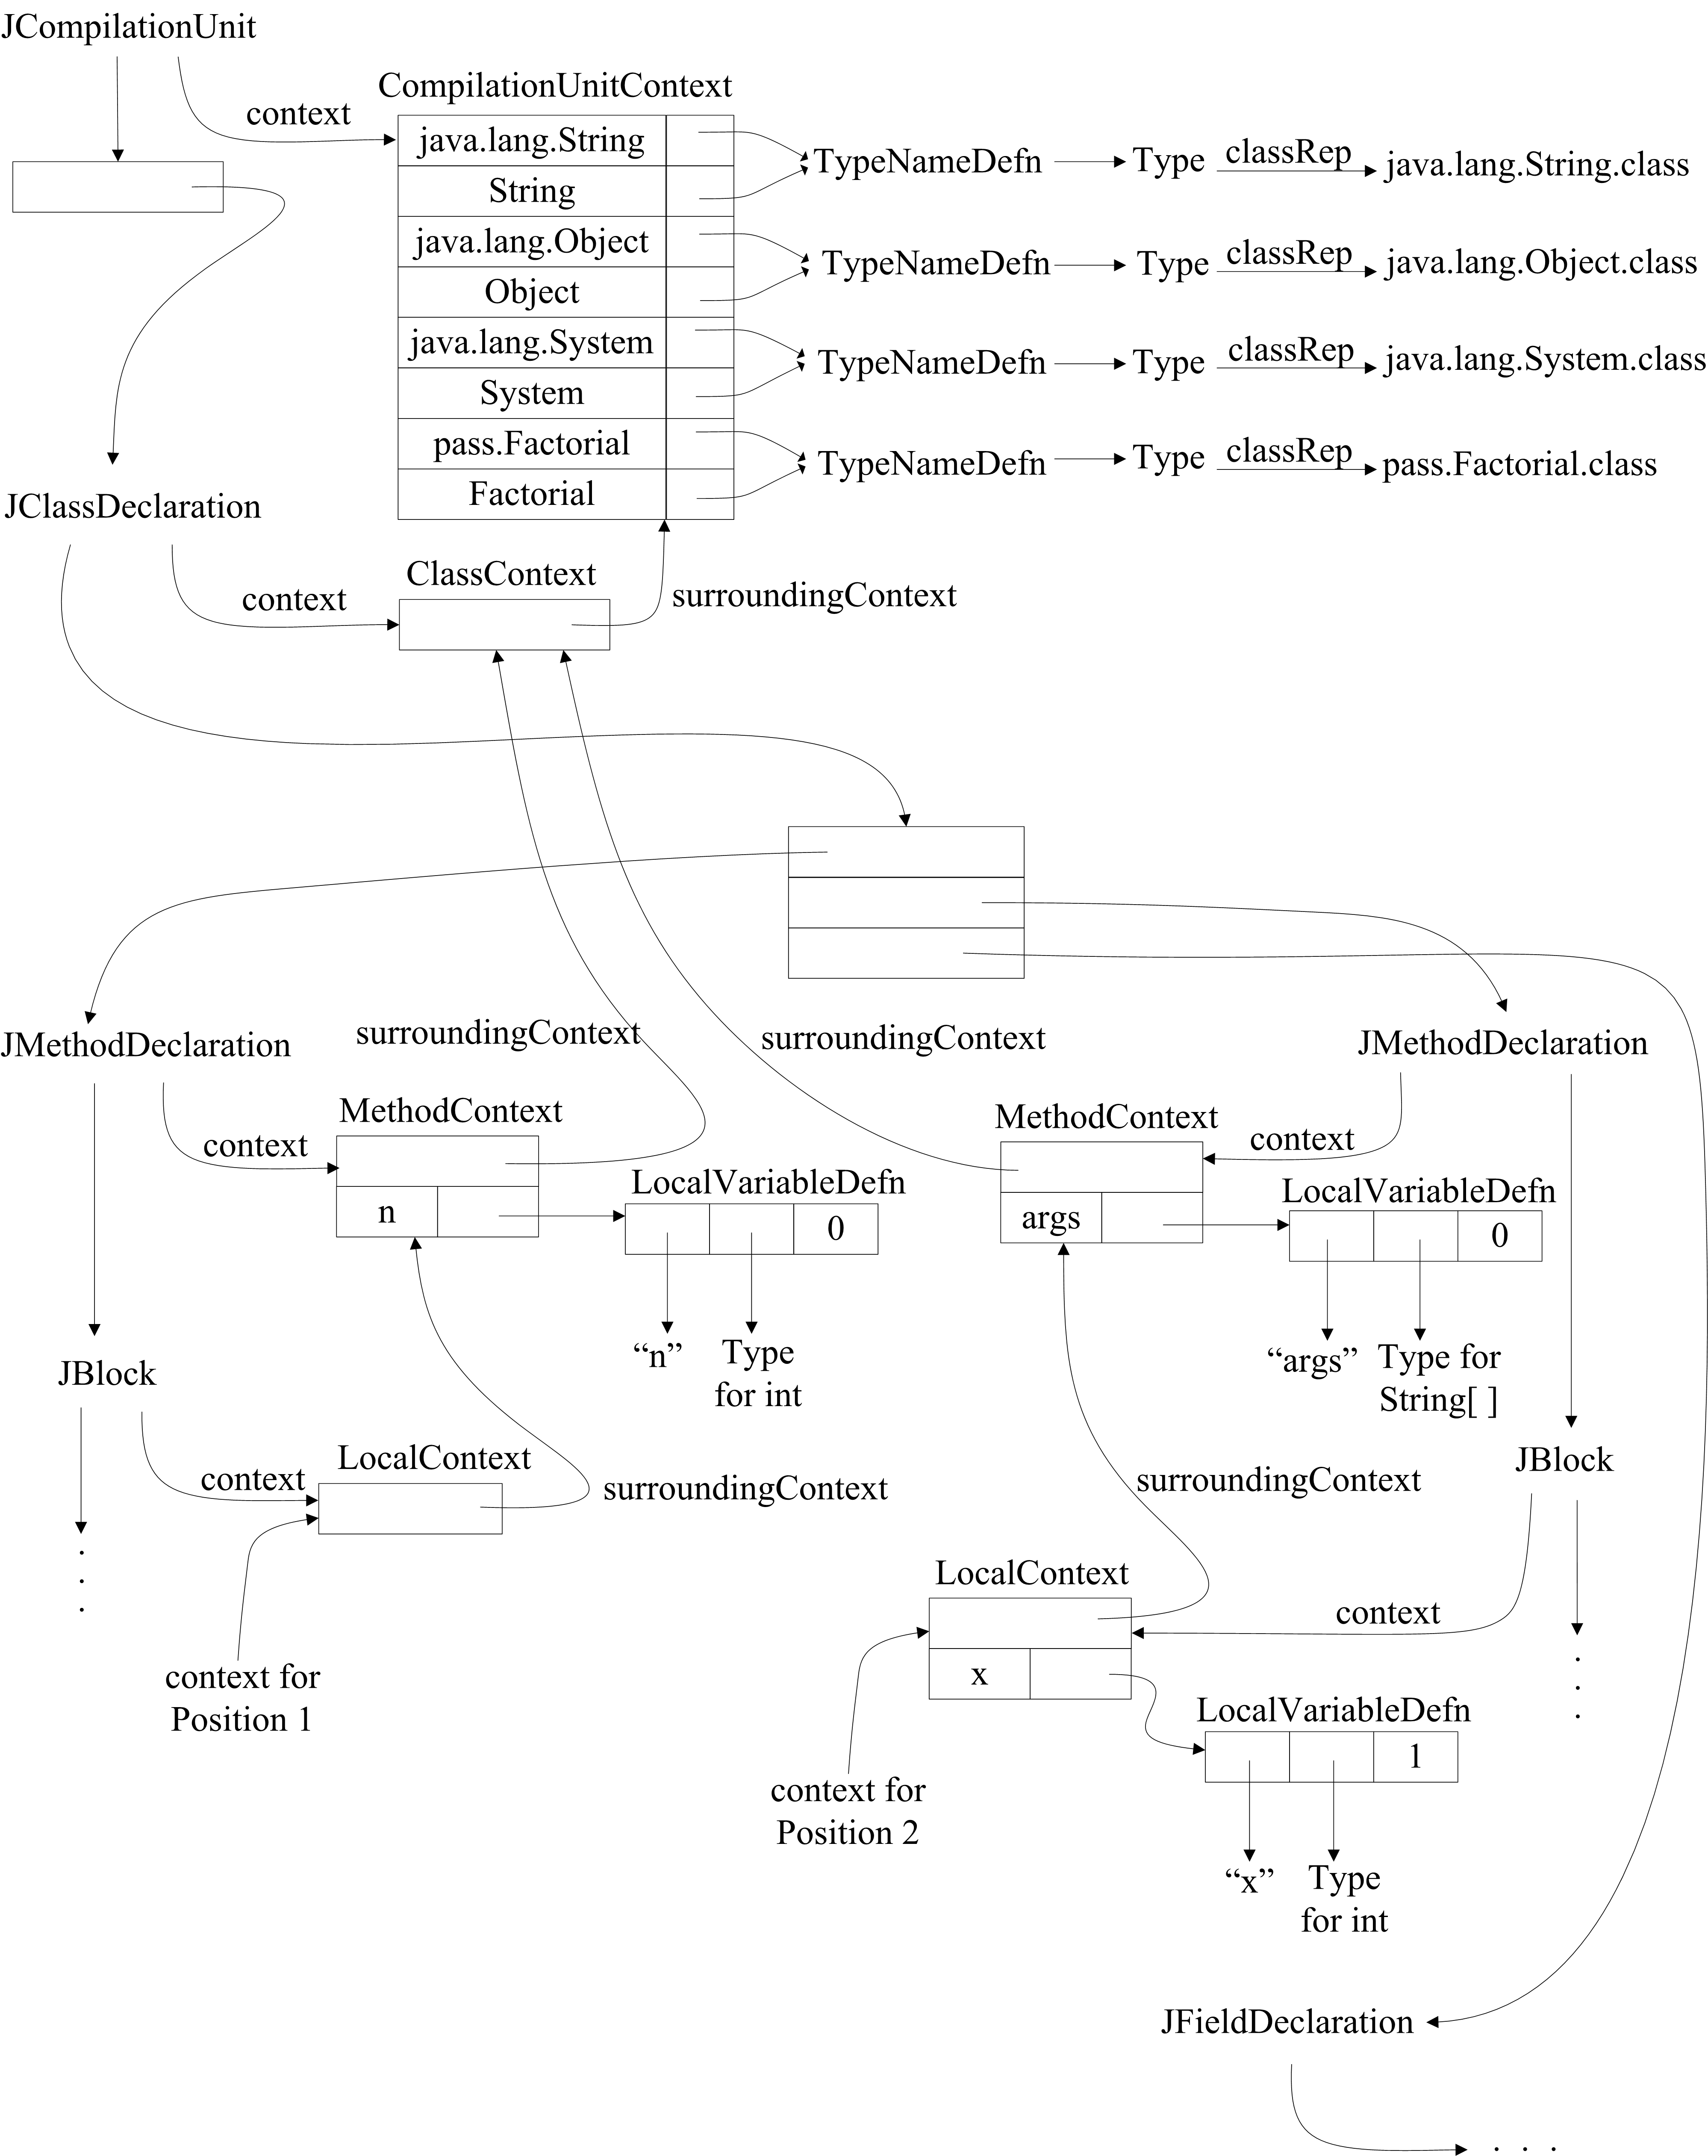
\includegraphics[scale=0.29]{{figures/figure04.01}.jpg}}
\end{center}
\end{frame}

\begin{frame}[fragile]
\pause

The symbol table takes the form of a tree that corresponds to the shape of the AST

\pause
\bigskip

A \lstinline{context}, ie, a node in this tree, captures the region of scope corresponding to the AST node that points to it

\pause
\bigskip

For example, in the above figure
\begin{enumerate}
\item The context pointer from the AST's \lstinline{JCompilationUnit} node points to the \lstinline{JCompilationUnitContext} that is at the root of the symbol table
\item The context pointer from the AST's \lstinline{JClassDeclaration} points to a \lstinline{ClassContext}
\item The context pointer from the AST's two \lstinline{JMethodDeclaration}s each point to a \lstinline{MethodContext}
\item The context pointer from the AST's two \lstinline{JBlock}s each point to a \lstinline{LocalContext}
\end{enumerate}

\pause
\bigskip

From any particular location in the program, looking back towards the root \lstinline{CompilationUnitContext}, the symbol table looks like a stack of contexts

\pause
\bigskip

Each \lstinline{surroundingContext} link back towards the \lstinline{CompilationUnitContext} points to the context representing the surrounding lexical scope
\end{frame}

\begin{frame}[fragile]
\pause

During analysis, when the compiler encounters a variable, it looks up that variable in the symbol table by name, beginning at the \lstinline{LocalContext} most recently created in the symbol table

\pause
\bigskip

Type names are looked up in the \lstinline{CompilationUnitContext}; to facilitate this, each context maintains three pointers to surrounding contexts, as illustrated in the following figure

\begin{center}
\visible<3->{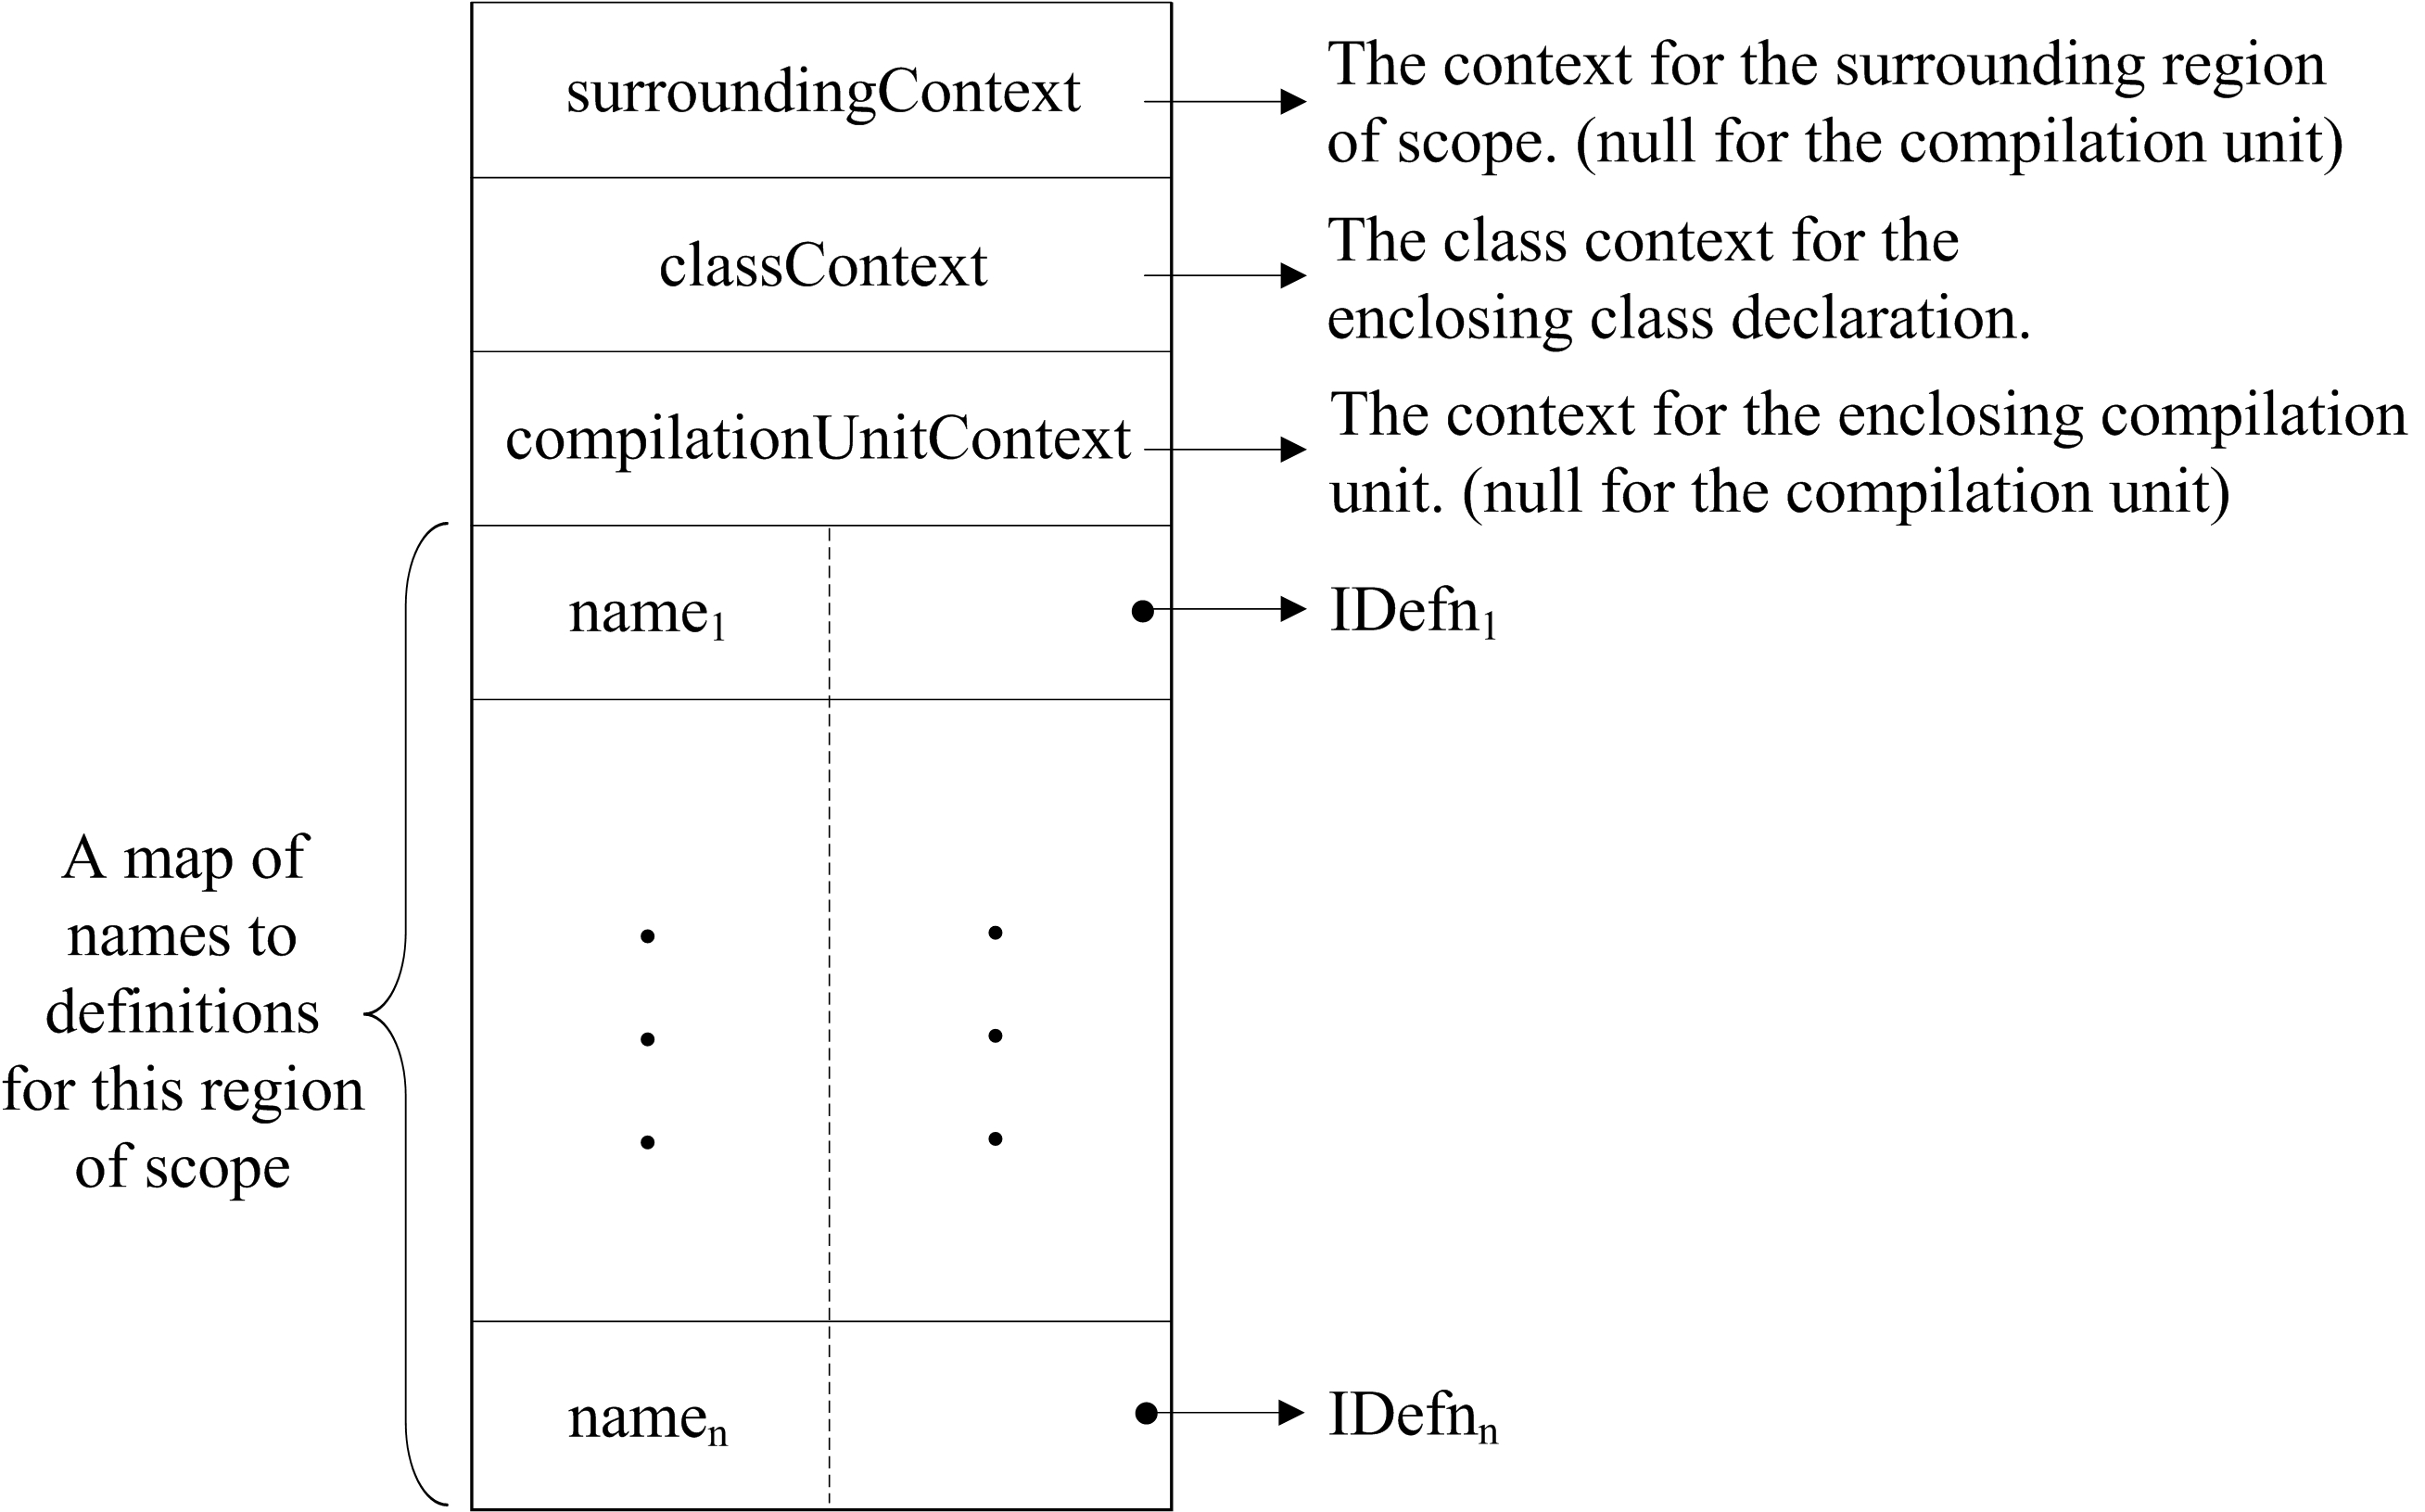
\includegraphics[scale=0.5]{{figures/figure04.02}.jpg}}
\end{center}
\end{frame}

\begin{frame}[fragile]
\pause

A \lstinline{CompilationUnitContext} represents the scope of the entire program and contains a mapping from names to types
\begin{itemize}
\item The implicitly declared types, \lstinline{java.lang.Object}, and \lstinline{java.lang.String}
\item Imported types
\item User-defined types, that is, types introduced in clss declarations
\end{itemize}

\pause
\bigskip

A \lstinline{ClassContext} represents the scope within a class declaration; in the \jmm symbol table, no names are declared here, but if we were to add nested type declarations to \jmm, they might be declared here

\pause
\bigskip

A \lstinline{MethodContext} represents the scope within a method declaration; a method's formal parameters are declared here

\pause
\bigskip

A \lstinline{LocalContext} represents the scope within a block, which includes the block defining the body to a method; local variables are declared here
\end{frame}

\begin{frame}[fragile]
\pause

Each kind of context derives from (extends) the class \lstinline{Context}, which supplies the mapping from names to definitions (\lstinline{IDefns})

\pause
\bigskip

The inheritance tree for contexts is illustrated in the following figure
\begin{center}
\visible<3->{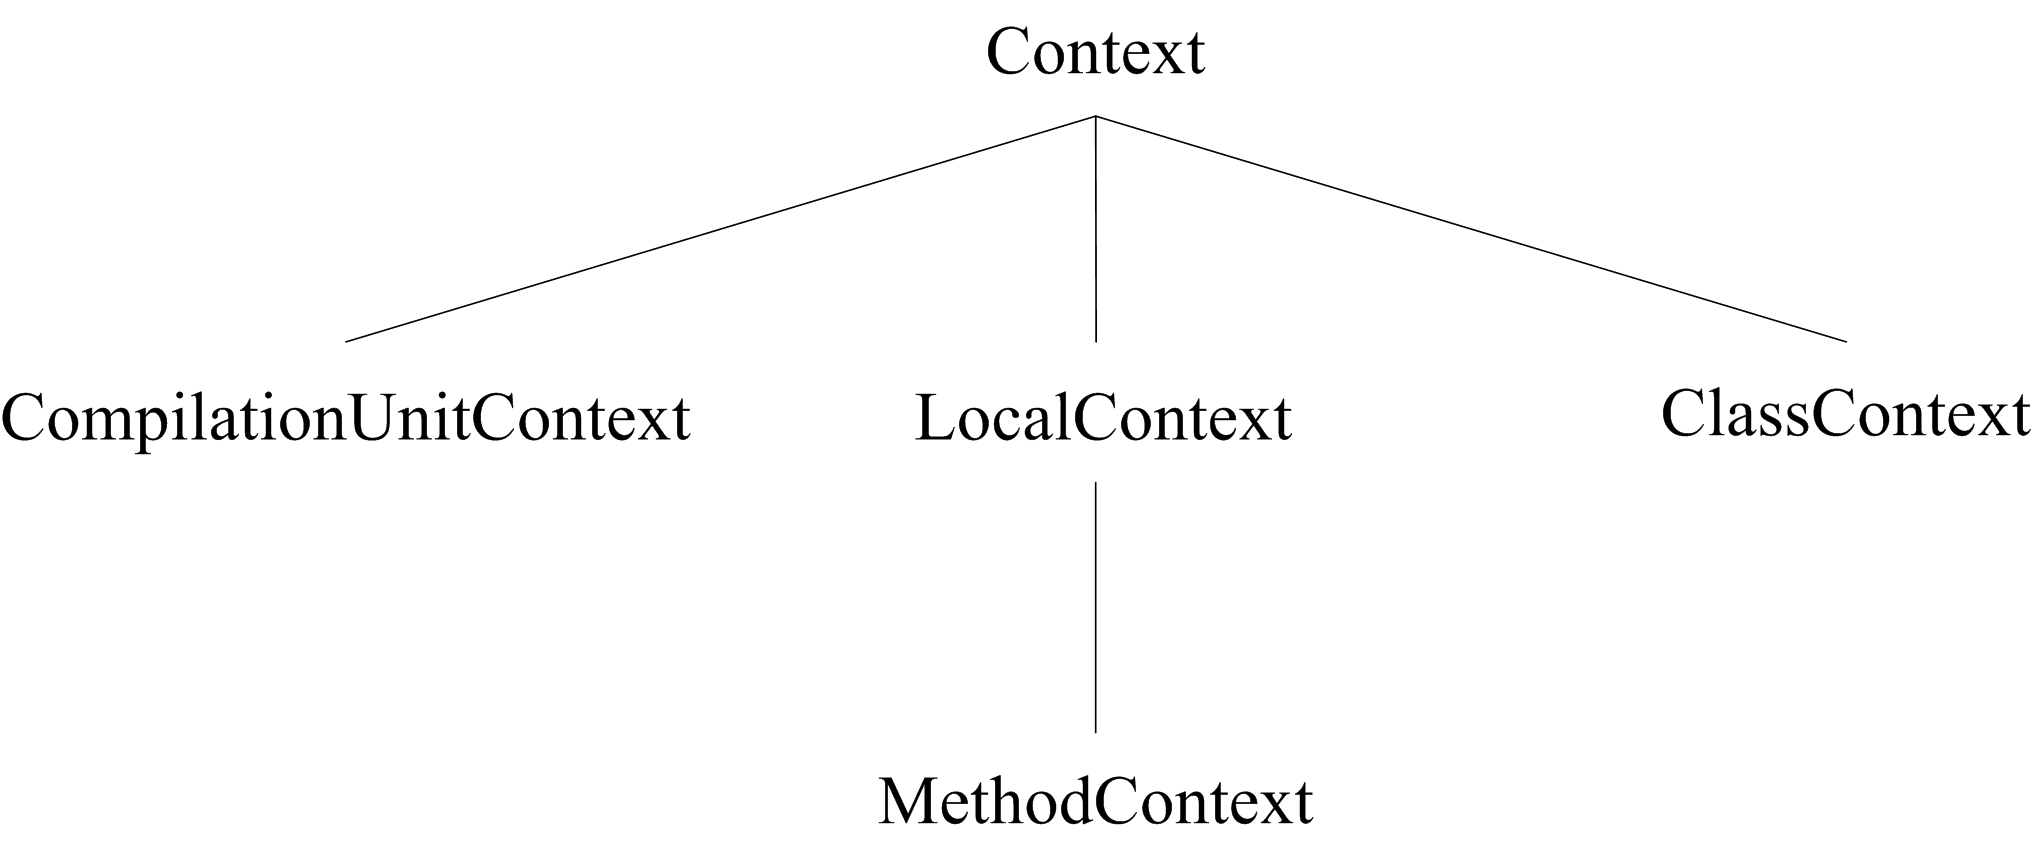
\includegraphics[scale=0.5]{{figures/figure04.03}.jpg}}
\end{center}

\pause
\bigskip

An \lstinline{IDefn} is the interface type for symbol table definitions, which has two implementations
\begin{enumerate}
\item A \lstinline{TypeNameDefn}, which defines a type name; an \lstinline{IDefn} of this sort encapsulates the \lstinline{Type} that it denotes
\item A \lstinline{LocalVariableDefn} defines a local variable and encapsulates the name, its \lstinline{Type} and an offset in the current run-time stack frame
\end{enumerate}
\end{frame}

\begin{frame}[fragile]
\pause

Class member (field and method in \jmm) names are not declared in a \lstinline{ClassContext}, but in the \lstinline{Type}s that they declare

\pause
\bigskip

We rely on the encapsulated \lstinline{Class} object to store the interface information, and we rely on Java reflection to query a type for information about its members

\pause
\bigskip

For example, \lstinline{Type} supports a method \lstinline{fieldFor()} which, when given a name returns a \lstinline{Field} with the given name that is defined for that type

\begin{lstlisting}[language=Java]
public Field fieldFor(String name) {
    Class<?> cls = classRep;
    while (cls != null) {
        java.lang.reflect.Field[] fields = cls.getDeclaredFields();
        for (java.lang.reflect.Field field:fields) {
            if (field.getName().equals(name)) {
                return new Field(field);
            }
        }
        cls = cls.getSuperclass();
    }
    return null;
}
\end{lstlisting}
\end{frame}

\section{Pre-analysis of \protect\jmm Programs}
\begin{frame}[fragile]
\pause


\end{frame}

\section{Analysis of \protect\jmm Programs}
\begin{frame}[fragile]
\pause


\end{frame}

\section{The Visitor Pattern and the AST Traversal Mechanism}
\begin{frame}[fragile]
\pause


\end{frame}

\section{Programming Language Design and Symbol Table Structure}
\begin{frame}[fragile]
\pause


\end{frame}

\section{Attribute Grammars}
\begin{frame}[fragile]
\pause


\end{frame}
\end{document}
